\documentclass{beamer}
\usepackage[T1]{fontenc}
\usepackage[utf8]{inputenc}
\usepackage[british]{babel}
\usepackage{verbatim}

%verbeek: pag 52 cap 3

% see https://tex.stackexchange.com/questions/68080/beamer-bibliography-icon/68084#68084 for reference
\usepackage[style=authoryear,dashed=false,backend=biber]{biblatex}
\usepackage{hyperref}

\setbeamertemplate{bibliography item}{%
	\ifboolexpr{ test {\ifentrytype{book}} or test {\ifentrytype{mvbook}}
		or test {\ifentrytype{collection}} or test {\ifentrytype{mvcollection}}
		or test {\ifentrytype{reference}} or test {\ifentrytype{mvreference}} }
	{\setbeamertemplate{bibliography item}[book]}
	{\ifentrytype{online}
		{\setbeamertemplate{bibliography item}[online]}
		{\setbeamertemplate{bibliography item}[article]}}%
	\usebeamertemplate{bibliography item}}

\defbibenvironment{bibliography}
{\list{}
	{\settowidth{\labelwidth}{\usebeamertemplate{bibliography item}}%
		\setlength{\leftmargin}{\labelwidth}%
		\setlength{\labelsep}{\biblabelsep}%
		\addtolength{\leftmargin}{\labelsep}%
		\setlength{\itemsep}{\bibitemsep}%
		\setlength{\parsep}{\bibparsep}}}
{\endlist}
{\item}

% general data
\title{Smart Home Ambient Intelligence: \\voice assistants}
\subtitle{\vspace*{0.3cm}a new limit for our freedom}
\author[Stefano Brandoli]{Stefano Brandoli}
\institute[PoliMi]{Politecnico di Milano\\Computer Ethics 2017/2018}
\date{December 12, 2017}

%theme and aspect
\setbeamertemplate{navigation symbols}{}
\addbibresource{bibliography.bib}
%\usetheme{metropolis}
\setbeamertemplate{section in toc}[circle]
\setbeamertemplate{subsection in toc}[ball unnumbered]
\setbeamerfont{subsection in toc}{size=\small}


\begin{document}

% frame
\begin{frame}
\maketitle
\end{frame}

% frame
\begin{frame}
\begin{center}\vspace*{-0.5cm}\textbf{Smart Home Ambient Intelligence: voice assistants\\a new limit for our freedom}
\end{center}
\frametitle{Presentation Outline}
\tableofcontents
\end{frame}

\section{Introduction}

% interleave
\begin{frame}
\begin{center}
	\usebeamerfont*{frametitle}
	\usebeamercolor[fg]{frametitle} Introduction
\end{center}
\end{frame}

\subsection{Technological Mediation}
% frame
\begin{frame}[fragile]
\frametitle{Technological Mediation}
\begin{quote}While fulfilling their function, technologies do much more: they \textbf{give shape to what we do} and how we experience the world. 
	And in doing so they \textbf{contribute actively} to the ways we live our lives (\cite{verbeek2011moralizing}, 12)
\end{quote}

\begin{itemize}
	\item Technologies are not \textbf{neutral intermediaries}
	%give shape to what we do and how we experience the world
	% turnstile, lightbulb, shopping cart coin, hotel keys
	\item Technologies play an \textbf{actively mediating role} 
	%in the relationship between human beings and reality. No autonomous subjects and mute and passive objects
	\medskip
	\item Artifacts are \textbf{bearers of morality} (\cite{latour1992})
	%as they help people to make all kinds of moral decisions
	% not in themselves but in relation to humans
	
	% example: obstetric ultrasound -> really morally charged
	% they help in moral decisions or they embed morality inside: even if morality requires intentionality and freedom

	\item Morality is a matter of \textbf{human-technology associations} (\cite{verbeek2011moralizing})
	% morality: not only per se but also as a consequence/interaction with artifacts: morality is a matter of human-technology associations

\begin{comment}
%	morality requires intentions and freedom: artifacts do not have them.
%	vs rigid separation of humans vs non humans in Latour words.
%	The only adequate way to understand it is in terms of its hybrid character.
%	it cannot be reduced to either an object or a subject but needs tobe understood in terms of their mutual relations. 
% Mediated action is not
amoral but is rather the preeminent place where morality finds itself in our
technological culture.
\end{comment}

\end{itemize}

\begin{itemize}
	\item Two perspectives of \textbf{technological mediation}:
	\begin{itemize}
		\item Perception
		% embodiment: glasses: see through
		% hermeneutic: like thermometer: requires interpretation
		\item \textbf{Action}: I will consider \textbf{human freedom}
		%Its central question is how human beings act in their world and shape their existence.
	\end{itemize}
\end{itemize}

\end{frame}

\subsection{Definitions}
% frame
\begin{frame}[allowframebreaks]
\frametitle{Definitions}	
	\begin{block}{Ambient Intelligence}
		\begin{quote}
			\textbf{Ambient Intelligence} is an approach that combines two major technologies: \textbf{Ubiquitous Computing} and \textbf{Intelligent User Interfaces (IUIs)} (\cite{brey2005freedom}, 158)
		\end{quote}
	\end{block}

	\begin{block}{Intelligent User Interface (IUI)}
		\begin{quote}
			Interfaces that allow combining mixed and \textbf{possibly ambiguous or imprecise input} (\cite{brey2005freedom})
		\end{quote}
	\end{block}

	\begin{block}{Voice Assistant}
		\begin{quote}
			A \textbf{voice assistant} is a digital assistant that uses \textbf{voice recognition}, \textbf{natural language processing} and speech synthesis to provide aid to users through phones and voice recognition applications (\cite{whatis})
		\end{quote}
	\end{block}
	\framebreak
	\begin{block}{Freedom}
		   Two forms (Brey 2005, 2006):
		   
			\begin{itemize}
				\item Negative Freedom:
					\begin{itemize}
						\item act without obstruction or interference by others
						\item absence of limits and \textbf{external constraints}
					\end{itemize}
				\smallskip
				example: artifact refusing to perform an action
				    \bigskip
					\item {\small \textbf{Positive Freedom (Human Autonomy)}:}
						\begin{itemize}
							\item mastery over your own life
							\item \textbf{think freely}, \textbf{make your own decisions} to act
							% and act based on those decisions
						\end{itemize}
			\end{itemize}
		\bigskip
		\textbf{I will consider freedom as human autonomy}
		
		% freedom enlarged instead of reduced? 
		% depends on the definition you consider, freedom in a more absolute concept (negative freedom) doesn't exist
		% giving you more possibilities and control in some particular situations
	\end{block}
\end{frame}

\section{Case Study: Google Home - Google Assistant Actions}

% interleave
\begin{frame}
\begin{center} 
	\usebeamerfont*{frametitle}
	\usebeamercolor[fg]{frametitle} Case Study: Google Home - Google Assistant Actions
\end{center}

\begin{figure}
	\centering
	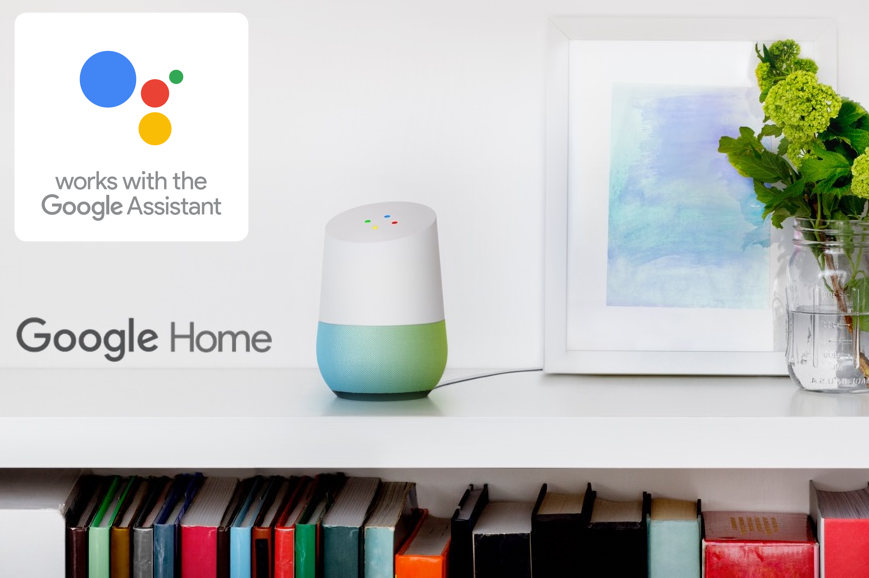
\includegraphics[width=1\linewidth]{images/Google-Home1}
	\label{fig:maxresdefault}
\end{figure}

\end{frame}

\begin{frame}
\frametitle{Case Study: Google Home - Google Assistant Actions}

\begin{columns}
	\column{0.45\linewidth}
	\begin{block}{Examples}
			\begin{itemize}
			\item Order a pizza
			\item Control devices in your home
			\item Many others \dots
		\end{itemize}
	\end{block}

	\column{0.55\linewidth}
	\begin{figure}
		\centering
		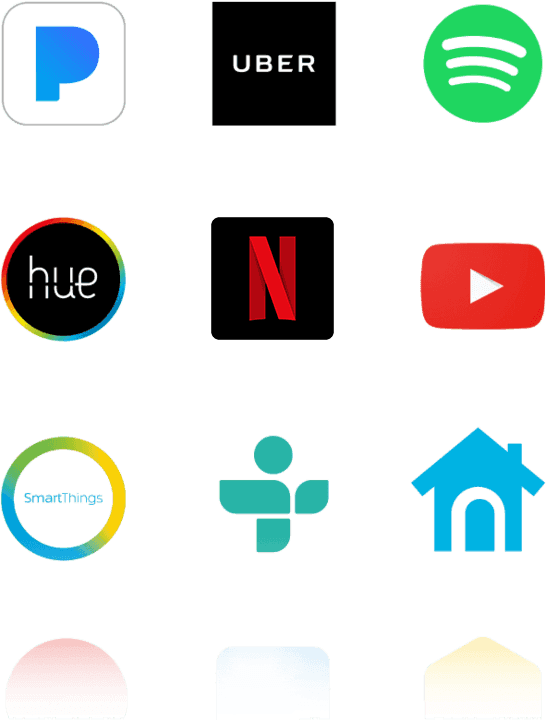
\includegraphics[width=0.7\linewidth]{images/logo-grid}
		\caption[Actions]{Google Assistant Actions}
		\label{fig:logo-grid}
	\end{figure}
	
\end{columns}

\end{frame}

% frame
\begin{frame}
\frametitle{Google Assistant Actions}
\vspace{-0.5cm}
\begin{figure}
	\centering
	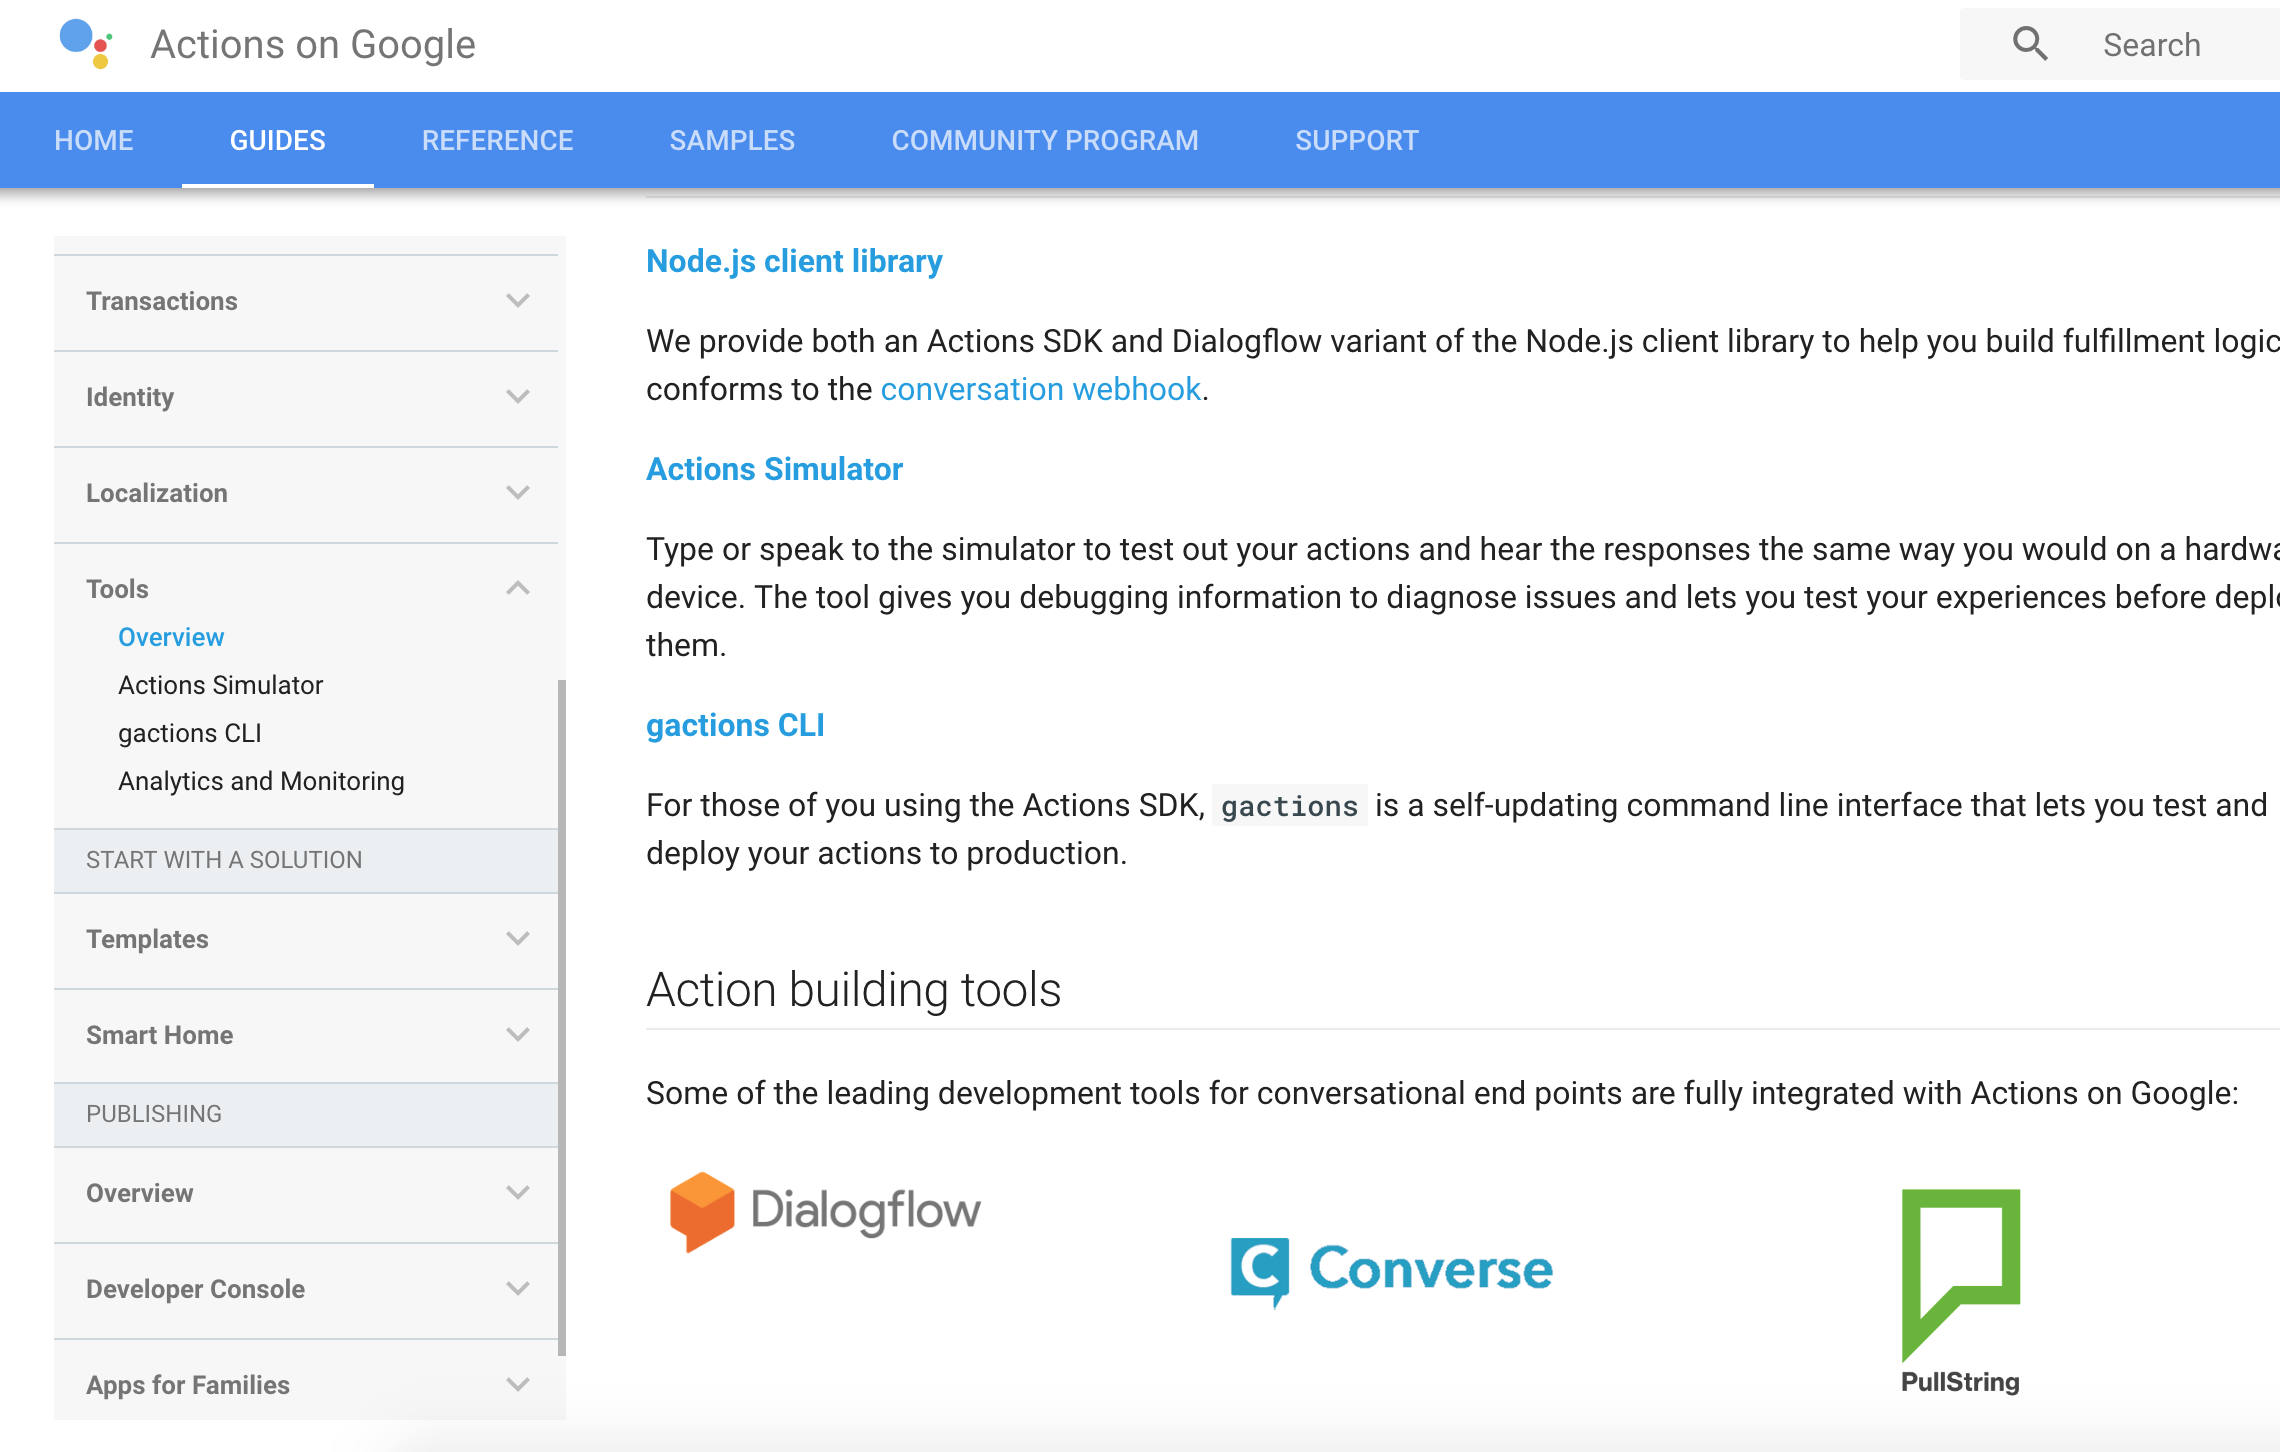
\includegraphics[width=0.85\linewidth]{images/documentation_preview}
	\label{fig:documentationpreview}
\end{figure}

% I Will Follow The Same Approach A Developer Follows When Dealing With New Technology
{\small Starting from the \textbf{Actions on Google documentation} I will show:
\begin{enumerate}
	\item \textbf{Applied concepts} of Technological Mediation \textbf{limiting freedom}
	\item \textbf{Ethical concerns} arising from \textbf{loss of freedom}
\end{enumerate}
}

\end{frame}

\subsection{Applied concepts of Technological Mediation limiting our freedom}
% interleave
\begin{frame}
\begin{center} 
	\usebeamerfont*{frametitle}
	\usebeamercolor[fg]{frametitle} Applied concepts of Technological Mediation\\limiting our freedom
\end{center}
\end{frame}

% frame
\begin{frame}
\frametitle{Script: make your own decisions}
% Developers design the whole conversational interaction.

\vspace{-0.3cm}
\begin{block}{Script} 
	\begin{quote}
		A \textbf{script} is a \textbf{prescription of  how to act} when using the artifact (\cite{verbeek2011moralizing})
	\end{quote}
\end{block}

Assistant Actions can be built (\cite{googleactions}):
\begin{enumerate}
	\item \textbf{With templates}
			%most of the app's conversation and fulfillment is handled by the template
			\begin{itemize}
				{\small  \item build apps \textbf{without writing a single line of code}
			 	 \item  build apps quickly \textbf{without worrying about designing conversations} }
		 	 	\smallskip
			 	 \item \textbf{Google decides} which interactions are good or not
		\end{itemize}
		
		\medskip
	\item \textbf{Without templates}
		\begin{itemize}
			\item \textbf{Dialogflow}
			% built-in natural language understanding: don't have to define a fully exhaustive grammar
		    % Extract the data you need from user input
				\begin{itemize}
					\item machine learning
					\item natural language understanding
					\item extract parameters (data) from the user vocal input
				\end{itemize}
			\smallskip
			\item \textbf{developers can decide} the whole conversational interaction
			% define what users can say to your app 
		\end{itemize}
\end{enumerate}

\end{frame}

\begin{frame}
\frametitle{Script: make your own decisions}
% speed bump
\begin{figure}
	\centering
	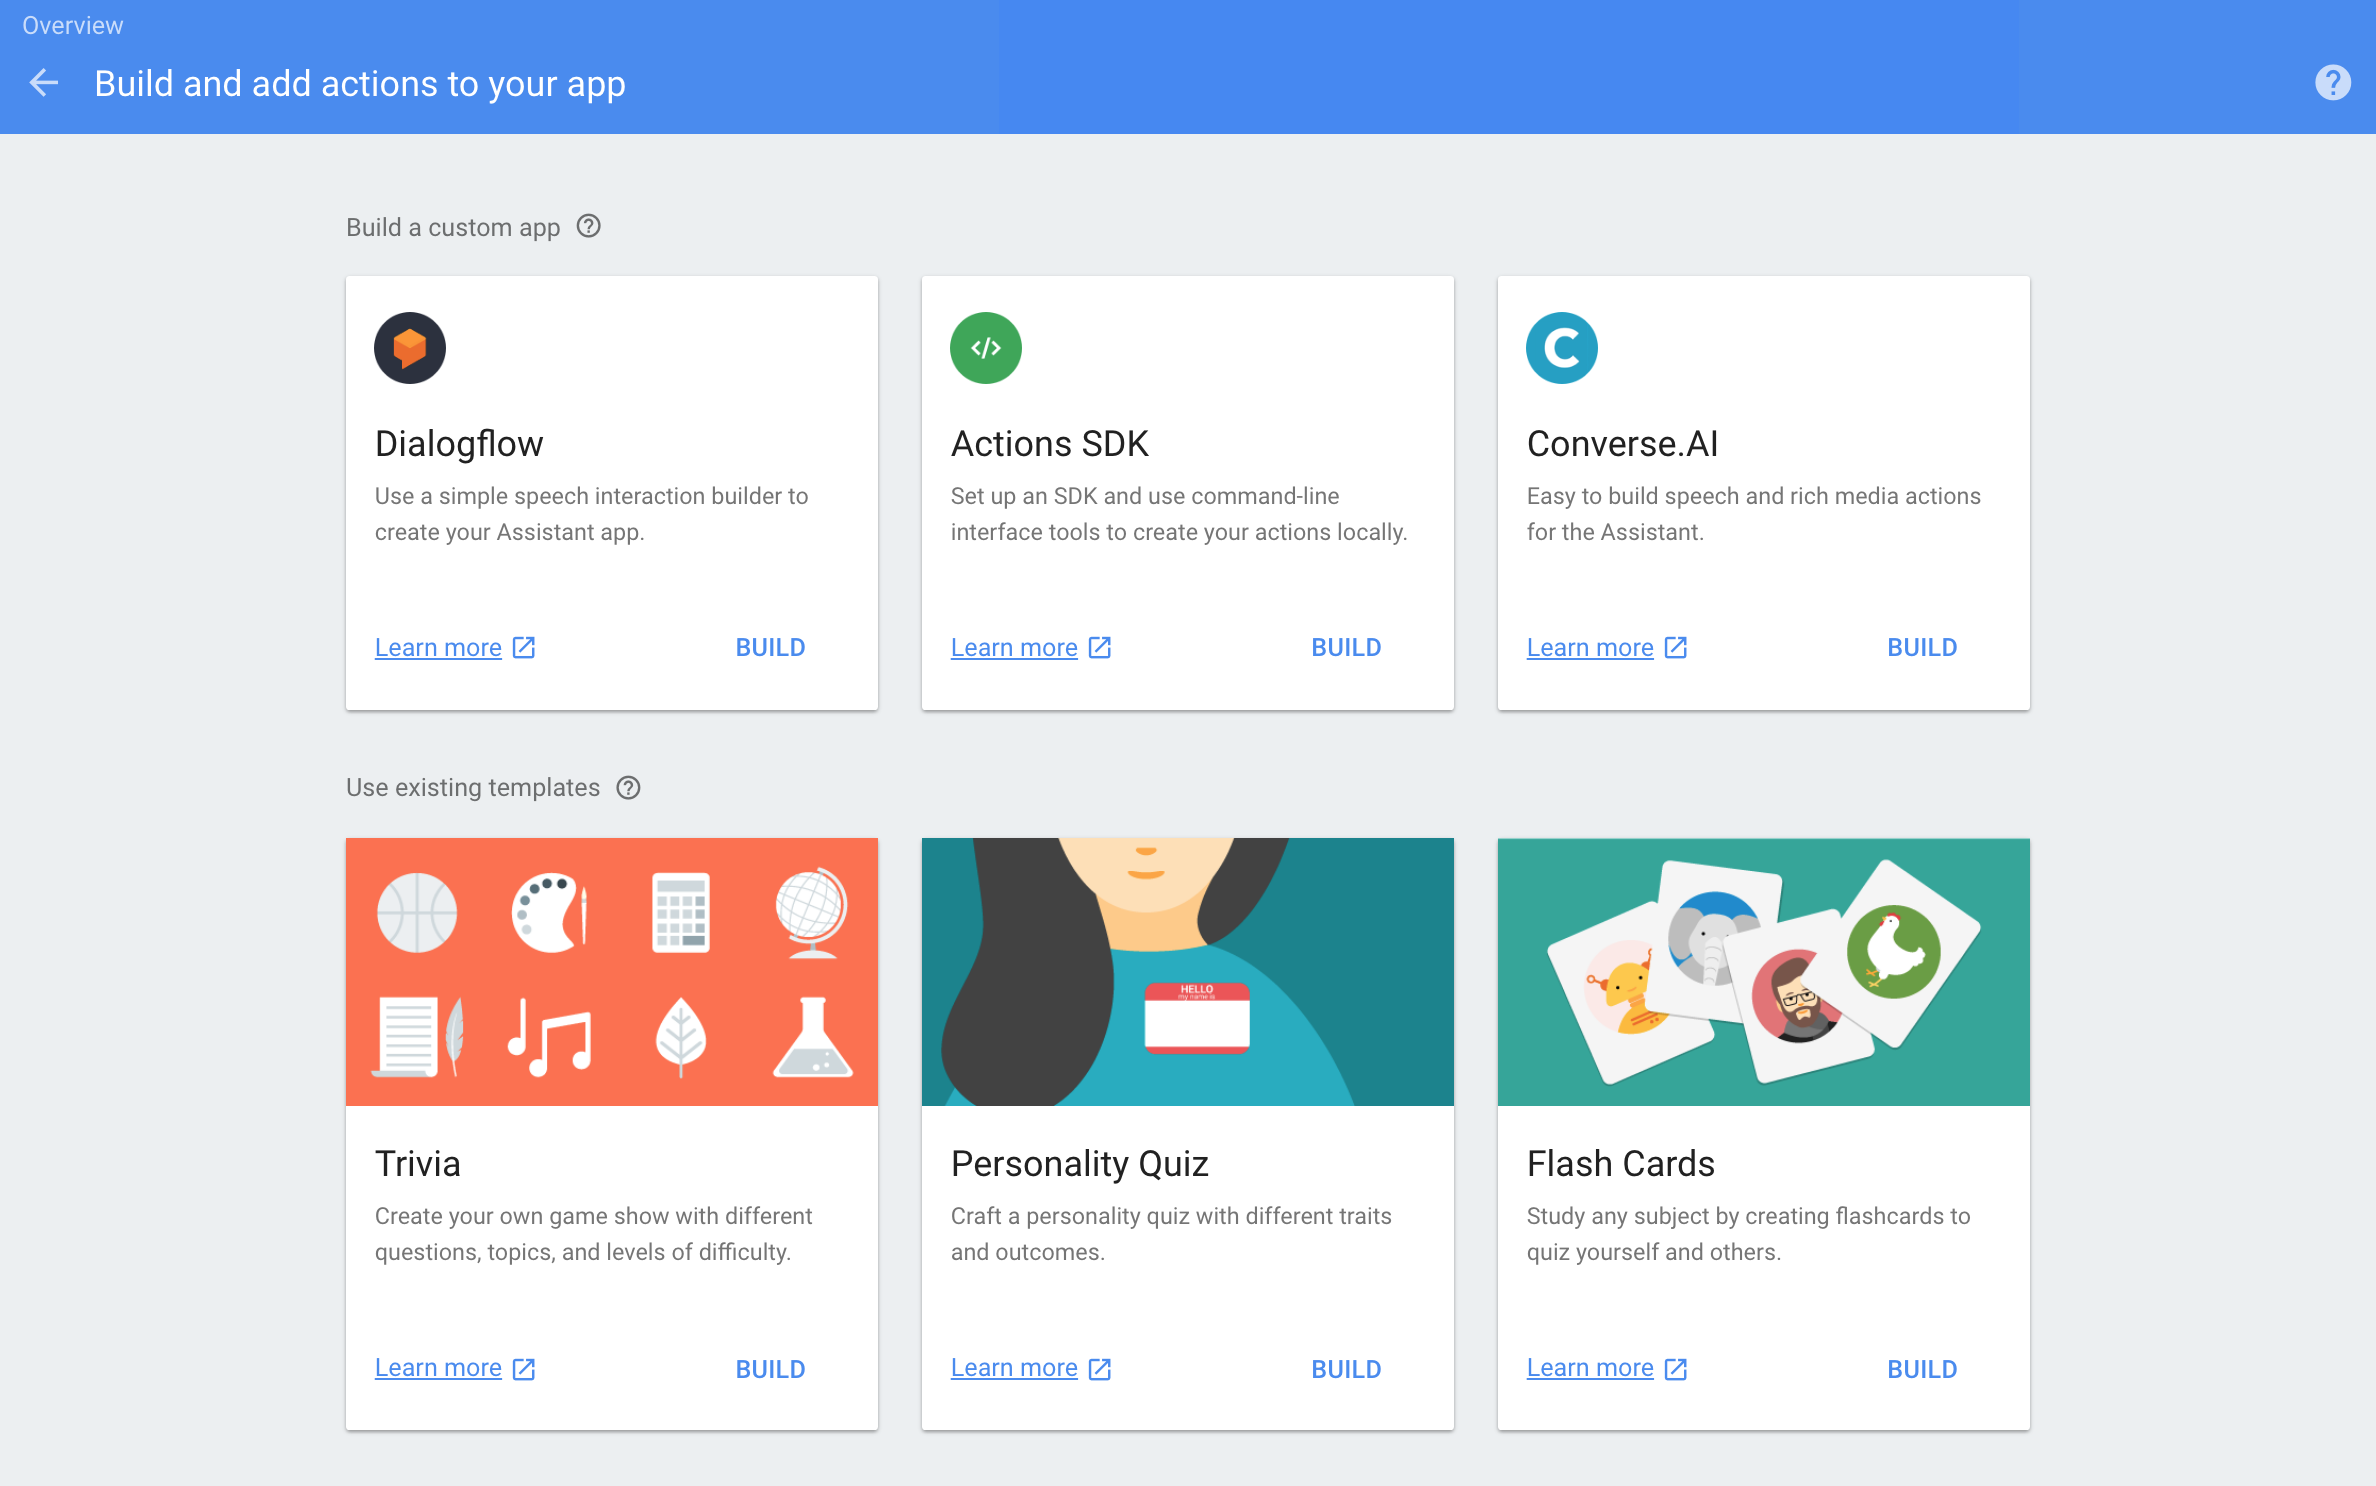
\includegraphics[width=1\linewidth]{images/script_image}
	\caption[actions_google]{Actions On Google Console}
	\label{fig:scriptimage}
\end{figure}

\end{frame}

% frame
\begin{frame}
\frametitle{Invitation/Inhibition: make your own decisions}
% Developers define what actions are possible and what are not. The scripts of artifacts suggest specific actions and discourage others. Idea: the flow won’t go on until the user has included in the answers the parameters

\begin{block}{Invitation/Inhibition} 
	\begin{quote}
		The scripts of artifacts \textbf{suggest specific actions} and \textbf{discourage others} (\cite{verbeek2011moralizing}, 21)
	\end{quote}
\vspace{0.5cm}
For the \textbf{Google Assistant Actions}:
\begin{itemize}
	% Fullfillment}
	% to respond to the user and to complete the requested action
	\item Developers while creating the application logic \textbf{enable some interactions} and \textbf{disable some others}
	% fulfillment
	% Dialogflow can extract parameters from the user input, validate the parameter and provide it to your fulfillment as a variable
	\item The \textbf{conversational interaction doesn't go on} if the user hasn't answered with \textbf{all the required parameters}
	%select the REQUIRED checkbox for the number parameter. This tells Dialogflow to not trigger the intent until the parameter is properly provided by the user.
\end{itemize}

\end{block}

\end{frame}

\begin{frame}
\frametitle{Invitation/Inhibition: make your own decisions}
\begin{figure}
	\centering
	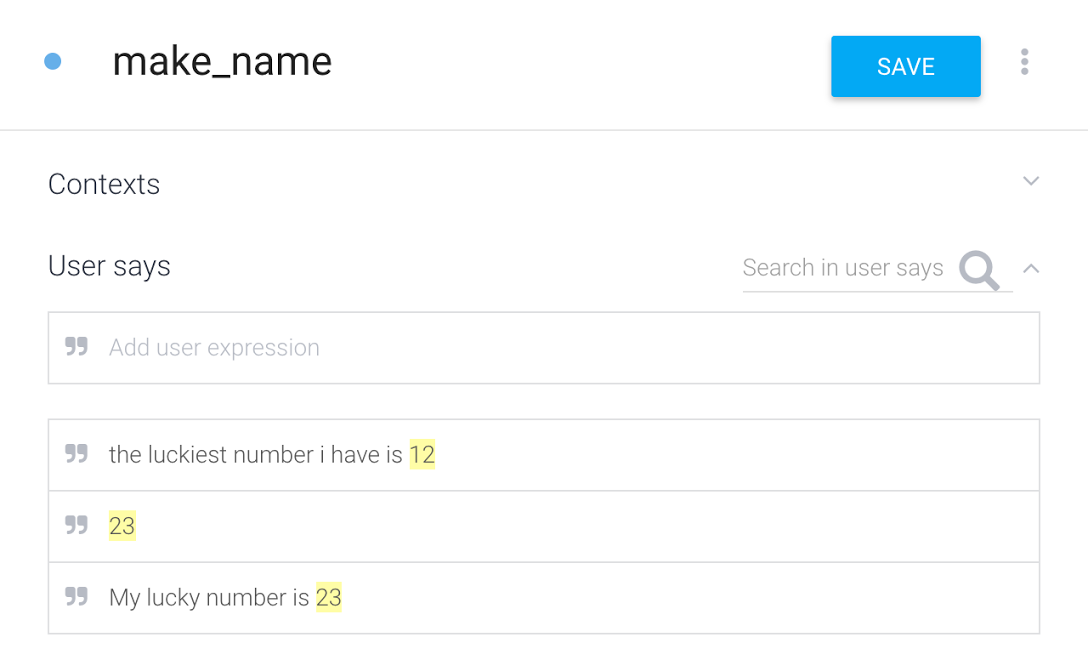
\includegraphics[width=0.75\linewidth]{images/invitation_inhibition}
	\label{fig:invitationinhibition}
\end{figure}

\begin{figure}
	\centering
	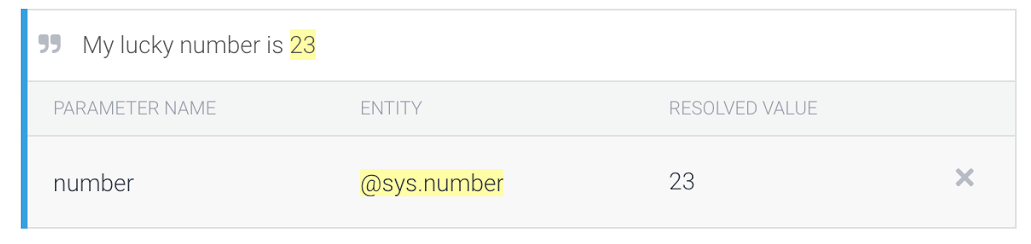
\includegraphics[width=0.7\linewidth]{images/invitation_inhibition_param}
	\label{fig:invitationinhibitionparam}
	\caption{DialogFlow interactions}
\end{figure}

\end{frame}

% frame
\begin{frame}[allowframebreaks]
\frametitle{Behaviour Steering: think freely}
%behaviour steer starts in our head and then leads to a steered action

	\begin{columns}
		\column{0.50\linewidth}
			\begin{block}{Suggestion Chips}
		 		\begin{quote}
		 			Use suggestion chips to \textbf{hint at responses} to continue or \textbf{pivot the conversation}\\(\cite{googleactions})
		 		\end{quote}
		 			
		 		%	If during the conversation there is a primary call for action, \textbf{consider listing that as the first suggestion chip} 
	 		\end{block}
 		\medskip
 		
 		\begin{itemize}
	 		\item This happens in vocal interactions
	 		\item \textbf{Can be more easily visualized on mobile phones}
	 	\end{itemize}
 	
		\column{0.50\linewidth}
			\centering
			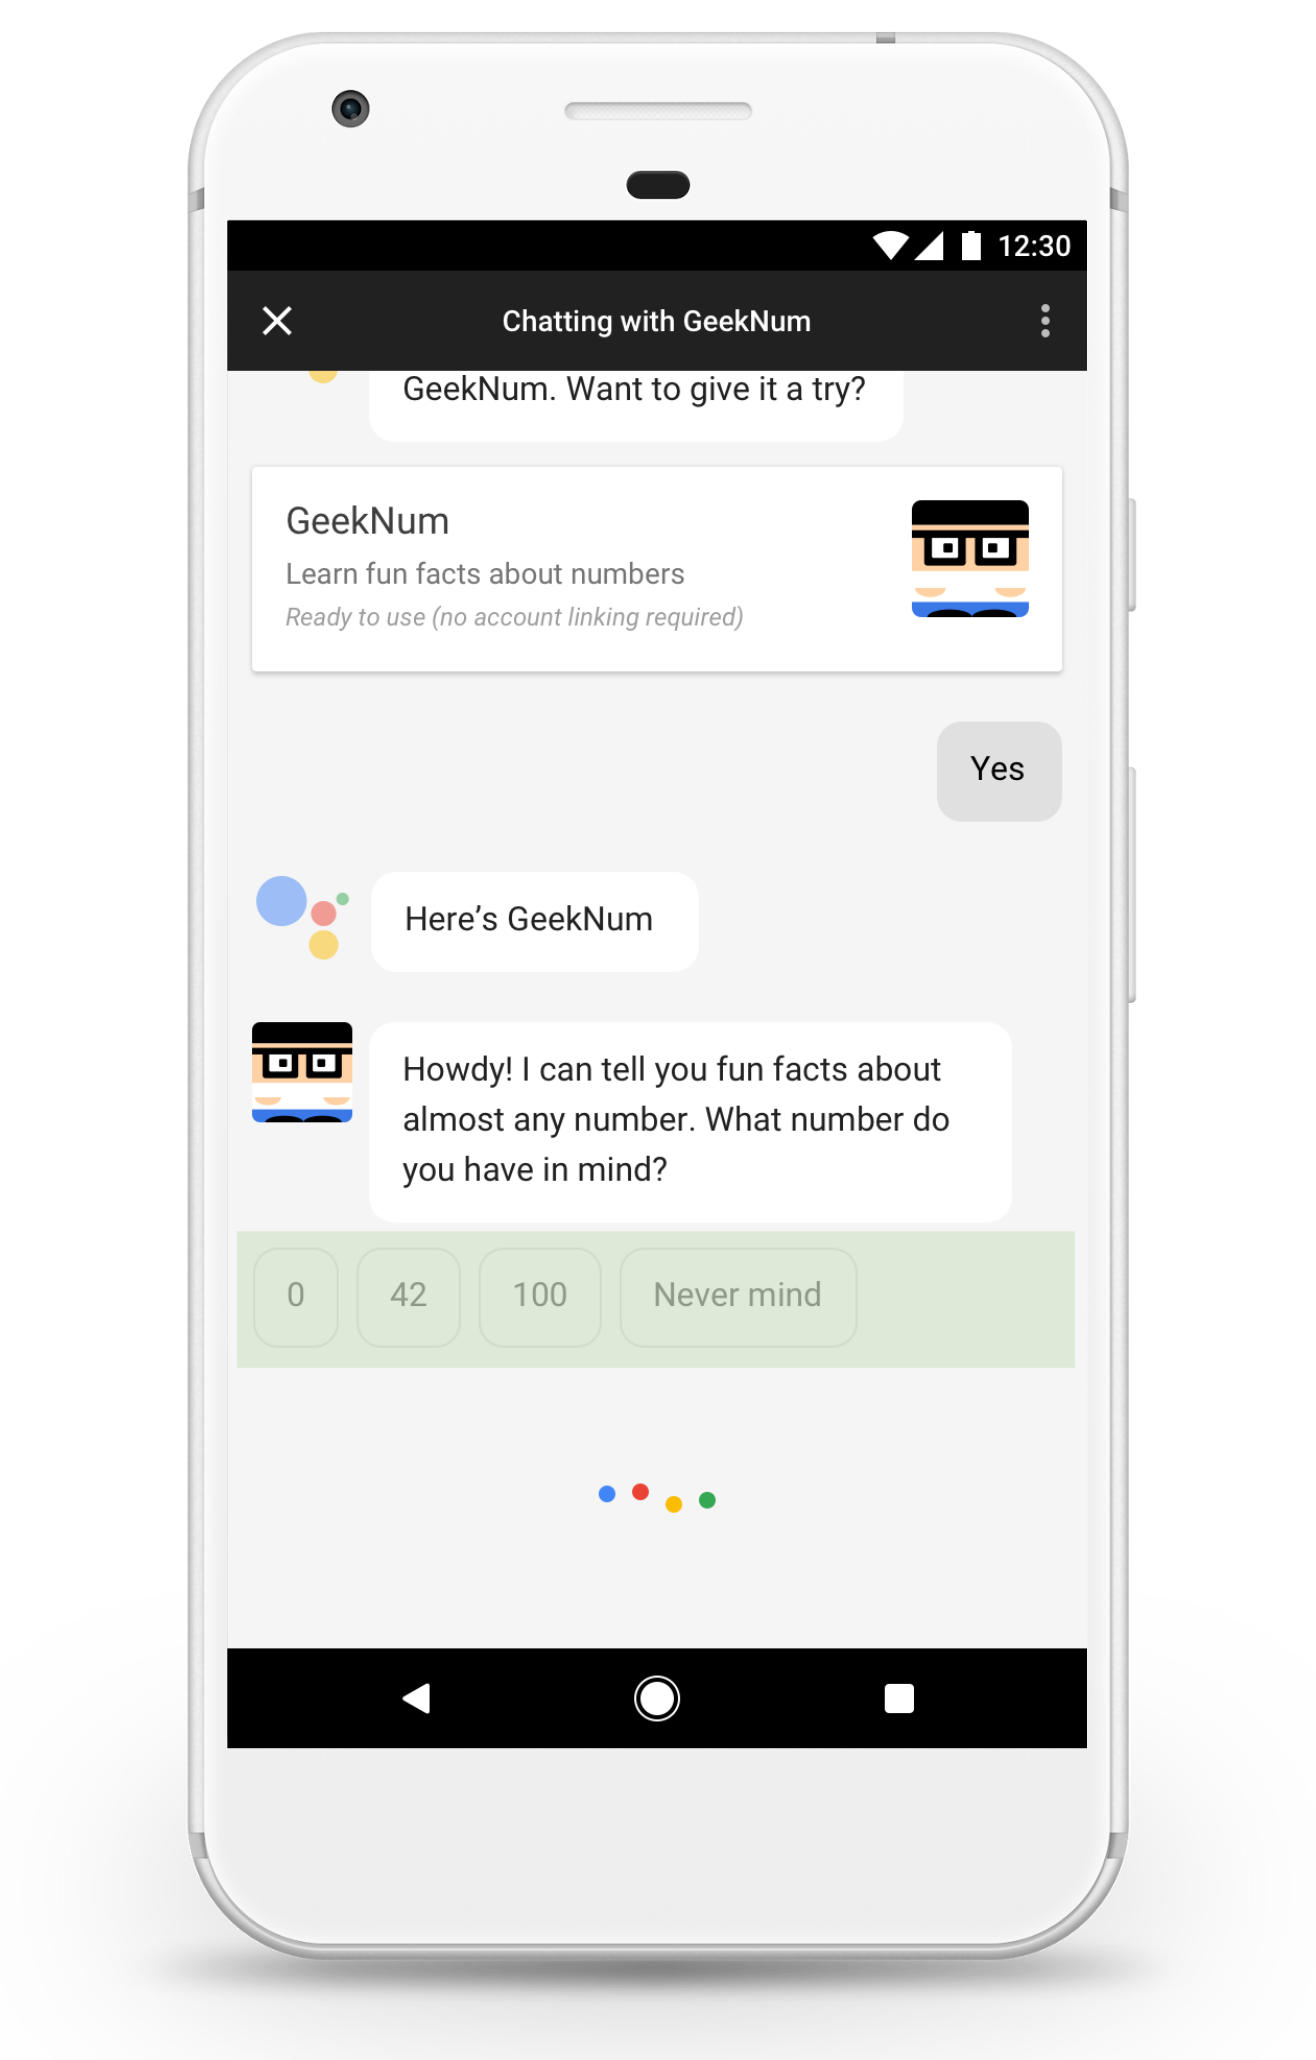
\includegraphics[width=1.05\linewidth]{images/suggestion-chip}
	\end{columns}
\framebreak

\begin{quote}
Smart objects could become \textbf{intermediaries between businesses and consumers}, using their intelligence to \textbf{persuade customers to buy products} \dots Such influence could already be \textbf{exerted at the design stage} \dots\\(\cite{brey2005freedom}, 163)
\end{quote}

\begin{block}{Advertisements}
	\begin{itemize}
		% in the middle of a normal answer to a user
		\item Google Assistant \textbf{advertised "\emph{Beauty and the Beast}"} film, but Google claimed it was not an ad (\cite{androidPolice})
		\medskip
		\item In future \textbf{Google Assistant will include ads}
			\begin{itemize}
				\item make money by \textbf{promoting e-commerce from partners} (\cite{recode})
				% Google’s vice president of ads division
				\smallskip
				\item forecasted ad-spend of \textbf{19 billions globally by 2022}
				%for voice assistants
				% 55% of all homes in the USA
				% About 70 Million Homes, Will Have Smart Speakers
				\\(\cite{juniper})
				\smallskip
				\item what if developers shape mediations based on \textbf{ads analytics}?
			\end{itemize}
	\end{itemize}
\end{block}

\framebreak
\begin{quote}
	\textbf{Agent-based dialogue systems} can be included in IUI’s

	to monitor users and \textbf{make assumptions about their intentions and the task they are trying to perform} \\(\cite{brey2005freedom}, 159)
\end{quote}

\begin{block}{Implicit Invocation}
\begin{quote}
The Assistant opts to invoke an app because it can fulfill the user's intent, \textbf{without users calling it by name} (\cite{googleactions})
\end{quote}
\vspace{-0.5cm}
\begin{figure}
	\centering
	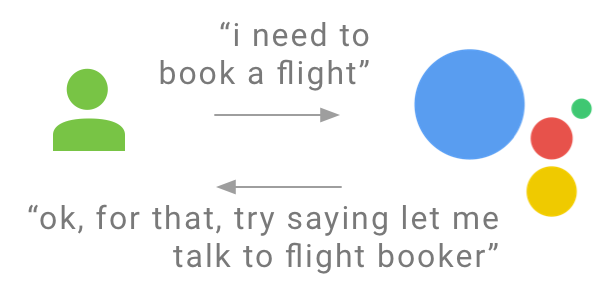
\includegraphics[width=0.55\linewidth]{images/implicit-invocation}
\end{figure}


%Users Will Commonly Learn About Your App Via The Assistant Directory, Which Is Like A Web Store For Apps On The Assistant.
\end{block}
\end{frame}

% frame
\begin{frame}
\frametitle{What about Technological Mediation?}
\vspace{-0.5cm}
\begin{figure}
	\centering
	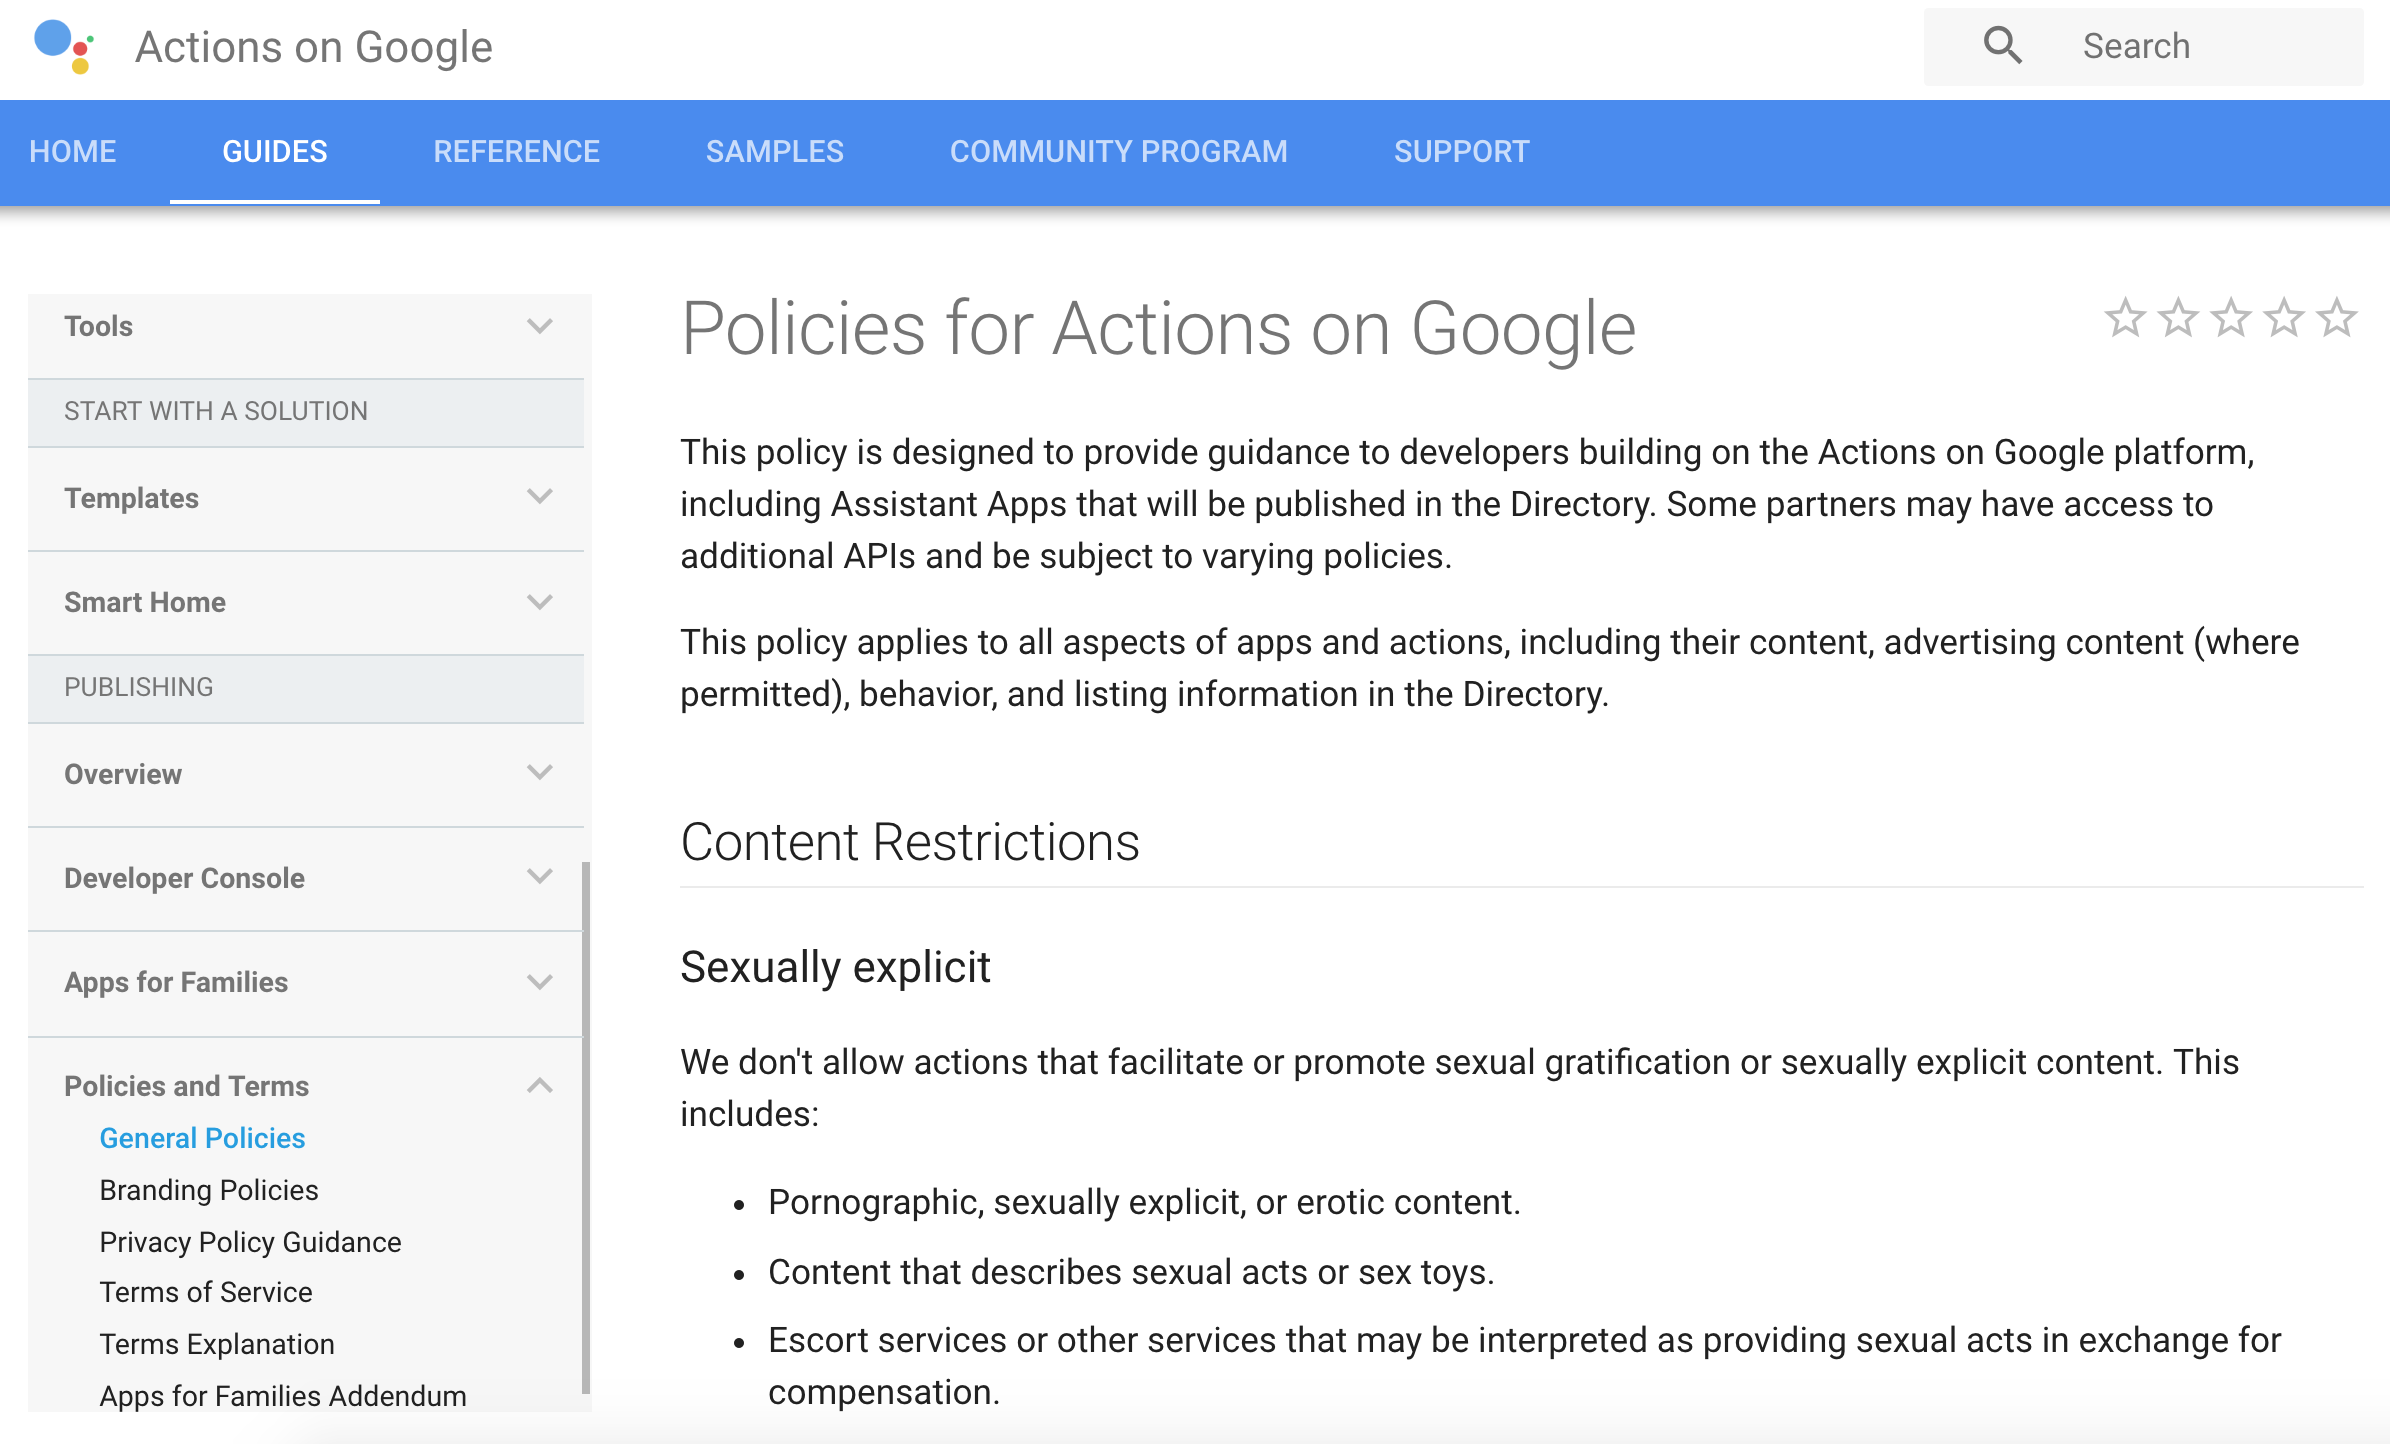
\includegraphics[width=0.95\linewidth]{images/dev_policy}
	\label{fig:devpolicy}
\end{figure}

\textbf{Google Actions Policies} are designed towards: privacy, content, branding \dots
\begin{itemize}
	% \item what about technological mediation?
	\item following the \textbf{Guidance For Conversation Design} is enough?
\end{itemize}
\end{frame}

\subsection{Ethical concerns arising from loss of freedom}
% interleave
\begin{frame}
\begin{center} 
	\usebeamerfont*{frametitle}
	\usebeamercolor[fg]{frametitle} Ethical concerns arising from loss of freedom
\end{center}
\end{frame}

% frame
\begin{frame}
	\frametitle{Fear of Technocracy}
	%If moral issues were solved through the technological activities of designers instead of the democratic activities of politicians, these critics averred, not humans but technologies would be in control

	\begin{itemize}
		\item \textbf{Experts} will shape our mediations
		\smallskip
		\begin{itemize}
			\item \textbf{Antidemocratic}
			% there is a danger that BSTs become undemocratic technologies, because their basic functionality may still be largely decided by engineers rather than by democratic representatives.
			%: because technocratic solutions are not democratic, and because they depend on the false idea that social problems can be solved by means of a technological ‘fix’
			\begin{itemize}
				\item How to make it more democratic?
				% both technologies and laws limit human freedom, but laws are democratically debated, while the moralization of technology is not
			\end{itemize}
			\smallskip
			\item \textbf{Unforeseen mediations}
			% technologies can be used in unforeseen ways and therefore have unforeseen influences on human actions. 
			\begin{itemize}
				\item Not humans but \textbf{technologies are in control}\\(\cite{verbeek2011moralizing}, 102)
			\end{itemize}
		\end{itemize}
	     \bigskip
		\item \textbf{Opposite problem}: people without enough technical background may design \textbf{Google Assistant Actions} and publish them
		\smallskip
		\begin{itemize}
			\item today are very limited mediations
			\smallskip
			\item \textbf{what about the future?}
		\end{itemize}
	\end{itemize}
\end{frame}

% frame
\begin{frame}
\frametitle{Moral Laziness}
\begin{itemize}
	\item Immorality or \textbf{amorality}
	\medskip
	\item People may \textbf{delegate all moral decisions to machines} \\(\cite{verbeek2011moralizing}, 134)
	\medskip
	\item \textbf{Commodification of morality} (\cite{borgmann1984technology})
		 \begin{itemize}
		 	\item Things that used to \textbf{require effort} to acquire have become
		 	available with the push of a button
		 	\smallskip
		 	\item today we don't even need buttons \dots
		 	\smallskip
		 	\item \textbf{voice assistants} are a new step in this process of commodification?
		 \end{itemize}
\end{itemize}
\end{frame}

% frame
\begin{frame}
	\frametitle{Moral Responsibility}
	\begin{itemize}
		\item Designing is \textbf{''materializing morality''} (\cite{verbeek2011moralizing}, 101)
		% designing mediations
		\bigskip
		\item To what extent \textbf{can designers be held morally responsible for undesirable forms of mediation}?\\(\cite{verbeek2011moralizing})
		\smallskip
		\begin{itemize}
			\item The responsibility should not be left to designers alone (\cite{verbeek2011moralizing})
			\medskip
			\item Google Actions Policies: \textbf{developers are the solely responsible for determining the legality} of their Actions
			\smallskip
			\begin{itemize}
				\item What about their \textbf{moral responsibility}?
				% causal responsibility vs moral responsibility
				%you can be the cause even if you are not moral responsible, in an accident for example
				% for moral responsibility you need to act with intentionality and freedom
				% this is more complex in technological mediation, moral responsibility stays in the middle
				% but this doesn't mean that we don't care, it's the opposite (we should care more)
				% so is in the middle between user, developer and artifact
				% several ways for designers to be morally responsible: assess, anticipate, design mediations
				% responsibility of the user: 
				% - accepts passibly the persuasions
				% - decides not be informed but still use the technology
				% - try to keep the control and do not rely only on those technologies
			\end{itemize}
		\end{itemize}
	\end{itemize}
\end{frame}

\section{Possible Remedies}
% interleave
\begin{frame}
\begin{center} 
	\usebeamerfont*{frametitle}
	\usebeamercolor[fg]{frametitle} Possible Remedies
\end{center}
\end{frame}

% frame
\begin{frame}
\frametitle{Possible Remedies}
\begin{itemize}
	\item Make the \textbf{design process more democratic} (\cite{verbeek2011moralizing})
	% mainly for the concepts of script and invitation/inhibition
	\smallskip
	\begin{itemize}
		\item Anticipate Mediation
		% CTA: socio ethical context
		\item Assess Mediation
		% try to assess (evaluate) the negative impacts a designed product may have in its use context
		\item Design Mediation
		% embed in the design of the object itself some moral mediations: this may limit human autonomy
		
		% rebound effect: technology designed for something but causing opposite effects: 
		%e.g. energy saving lightbulb increasing energy consumption
		% e.g. washing machines more energy efficient, used more times for small cloth quantity
	\end{itemize}
	\medskip
	\item Teach managers and voice assistants' developers to \textbf{think about Technological Mediation} and \textbf{the limits to our freedom}
	% mainly for behaviour steering
	\medskip
	\item Re-think the \textbf{moral responsibility of designers} of voice assistant actions
	% in my opinion in this case the moral responsibility is not in the middle between user, artifact and designers but is most on the developer side, there we need to make improvements
\end{itemize}
\end{frame}

% bibliography frame,see https://tex.stackexchange.com/questions/68080/beamer-bibliography-icon/68084#68084 for reference
\nocite{*}
\begin{frame}[noframenumbering,plain,allowframebreaks]{References}
\renewcommand*{\bibfont}{\small}
\printbibliography
\end{frame}

\end{document}